% Copyright (c) 2014,2016 Casper Ti. Vector
% Public domain.

\chapter{交易模型分析}
%\pkuthssffaq % 中文测试文字。
在設計一個区块链的实名交易监督系统之前,必須要針對不同的交易模型做探討。
在本密碼貨幣的商家收銀金流監控系統中,會以密碼貨幣的觀點重新設計一個新的支付系統,重新深究匿名者與匿名者之間的交易模式、實名與實名之間的交易模式、匿名與實名之間的交易模式,這三種交易模式所代表著意義與時代革新帶來的技術變革。
%%fig allan
\begin{figure}[h]
	\centering
	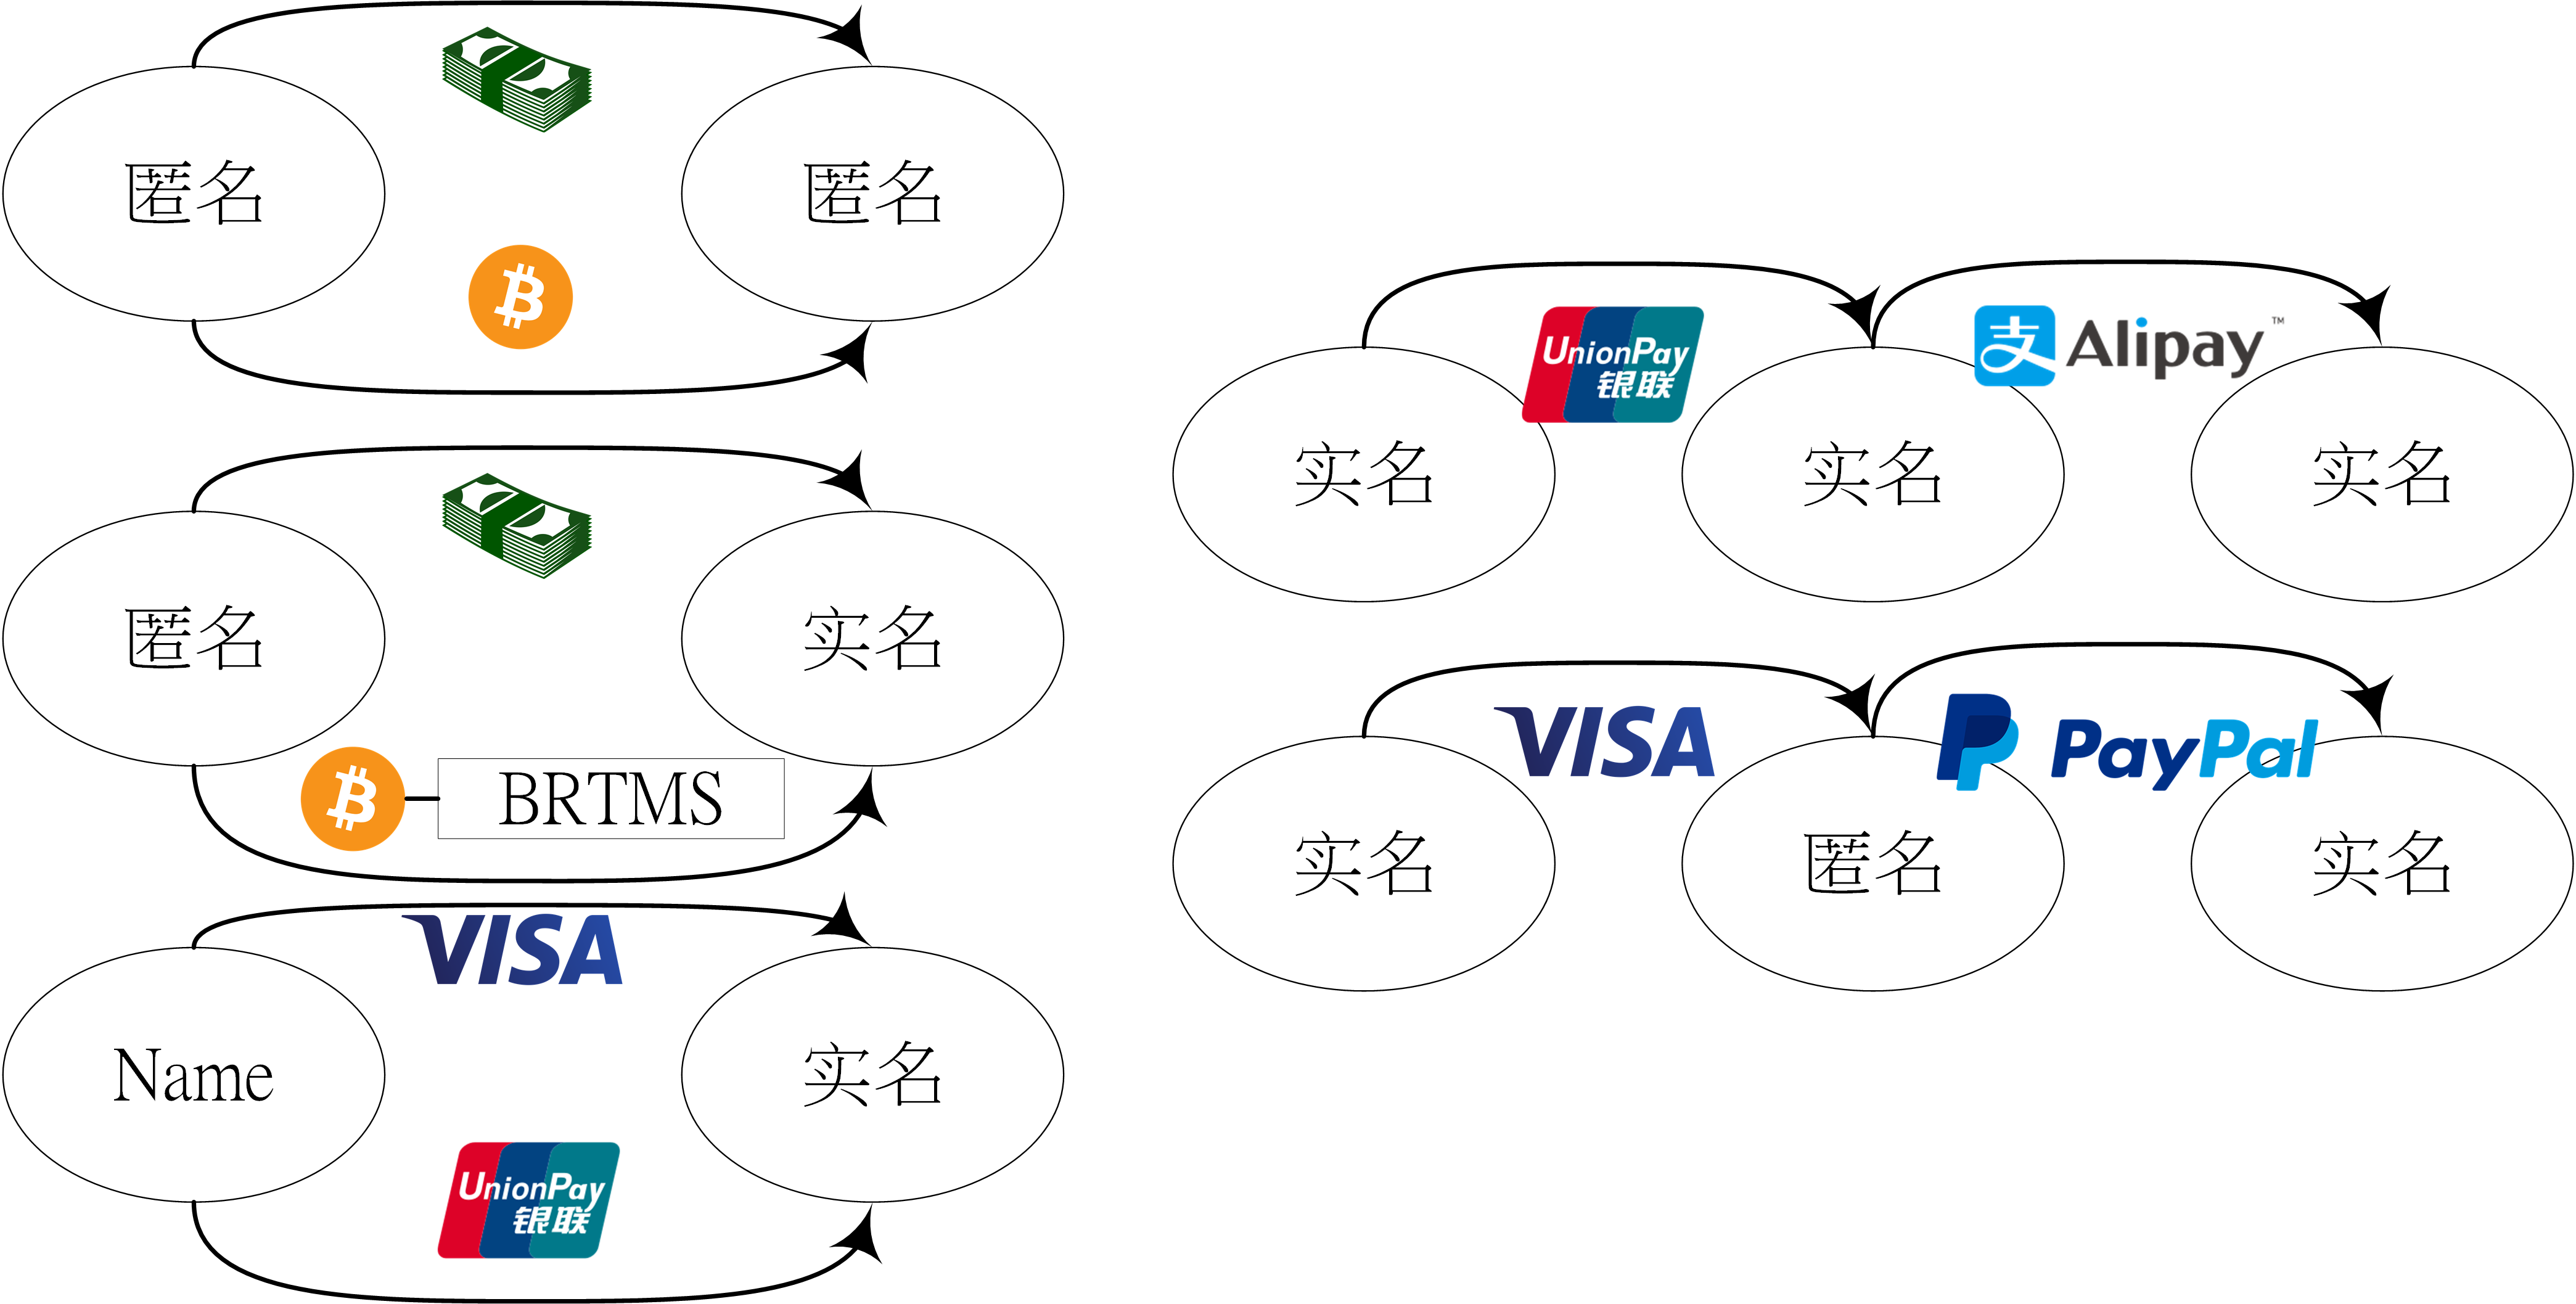
\includegraphics[width = 0.8\textwidth]{modeall.png}
	\caption{modeall}\label{modeall}
\end{figure}

	\section{現金交易模型}
		\subsection{匿名客戶對匿名商家}最早人類的交易行為可以探究到以物易物的交易行為模式,進而發展出銅幣、紙幣、金幣,甚至是現今常聽聞的金本位制度。 
		在交易的過程中商家無法知道消費者的真實身分,而在一些沒有收據的環境下,如雜貨店或是攤販、一些沒有開收據的商店,消費者也不知道商家的真實身分,故將此交易模式定義為”匿名者與匿名者之間的交易模式”。在這樣的交易模式下,消費者保持匿名,對消費者而言,可以有效的保護消費者的個人資訊安全,因為在貨幣的持有的方式,並不需要登記姓名,資產轉移的過程中一不需要。對於消費者而言,雖然消費者的匿名保護了自己的個人資訊,但商家的交易資訊也是匿名,對整個交易結果若有爭議,這便是追訴無門的結果。而在交易並未被有效紀錄的情況下,政府對稅收的計算,會進入無法計算的灰色地帶。圖\ref{modeaa}為匿名的消費者對未開立收據或是實名制的商家的交易模型。

		\begin{figure}[h]
			\centering
			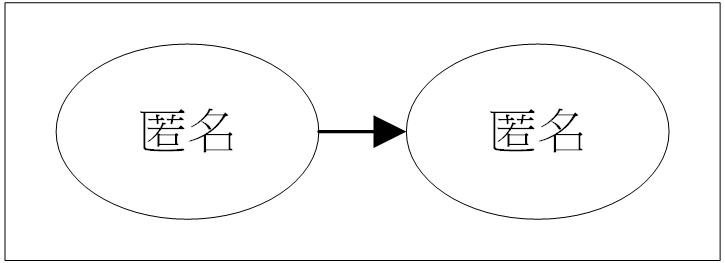
\includegraphics[width = 0.4\textwidth]{modeaa.png}
			\caption{匿名對匿名交易}\label{modeaa}
		\end{figure}

		%%%%%%%fig modeaa

		\subsection{匿名客戶對實名商家}
		在另一個場景中,在交易進行的過程中,消費者為匿名,商家俱有實名,對消費者而言因為自己本身並無綁定個人資訊,故對各資隱私有很大的保障,消費者消費的物件店家具有實名而開立收據,對消費者而言會得到消費紀錄的保障,對消費的糾紛有店家可以追溯。對政府,因為交易的紀載史的稅收的計算變得容易。圖\ref{modean}為消費者使用現金隊已經實名制或是開立收據的商家消費的模型。

		\begin{figure}[h]
			\centering
			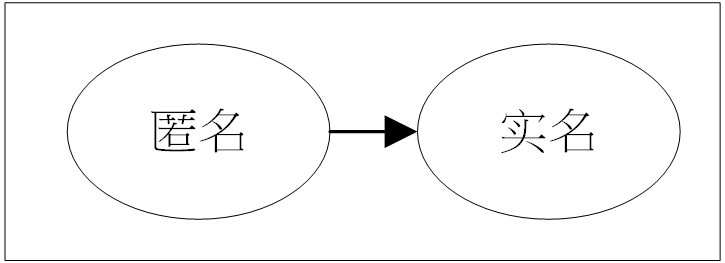
\includegraphics[width = 0.4\textwidth]{modean.png}
			\caption{匿名對實名交易}\label{modean}
		\end{figure}

		%%%%%%%fig an

	\section{電子貨幣交易模型}
		\subsection{實名客戶支付實名商家}
		在現在最為常見的塑膠貨幣支付管道Visa中,因為當年的設計並無類似區塊鏈去中心化的理論、技術提出,因而資金的轉移設計會是銀行帳戶與銀行帳戶間的資金轉移,也因為這樣的設計,造成交易的基礎被規範在實名與實名之間的交易模式,這樣的交易模式,雖然快速且方便,但在無形之中透漏了許多消費者的個人資料。在交易手續費方面,Visa的手續在跨國刷卡的場景下,皆需要收取高達百分之一點五的手續費,對於消費者而言使用VISA作為支付會帶來不小的負擔。圖\ref{modenn}為透過實名制支付管道對商家進行交易的模型。

		\begin{figure}[h]
			\centering
			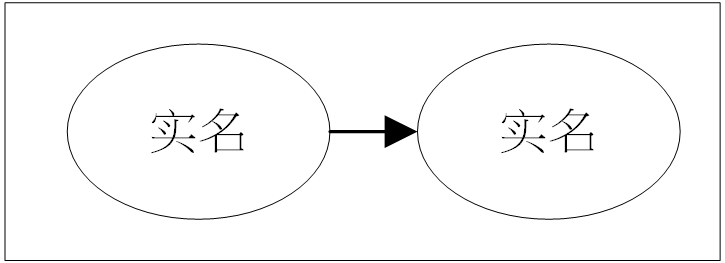
\includegraphics[width = 0.4\textwidth]{modenn.png}
			\caption{實名對實名交易}\label{modenn}
		\end{figure}

		%%%%%%%fig nn


		\subsection{實名客戶透過實名第三方再實名商家}
		在中國VISA較不為常見,但除了VISA電子支付還有中國本身自營的銀聯,但因為中國的銀行眾多林立,且在科技化的世代中隨身帶著許多的卡片會造成相當不便,所以支付寶致力於將所有的卡片電子化,將所有中國在的銀行卡統合在一起,如此的集成所有的銀行卡的工作,可以有效的讓卡片交易更加的方便,圖\ref{modennn}為以實名制的銀聯卡透過支付寶進行支付給實名制的店家的交易模型。

		\begin{figure}[h]
			\centering
			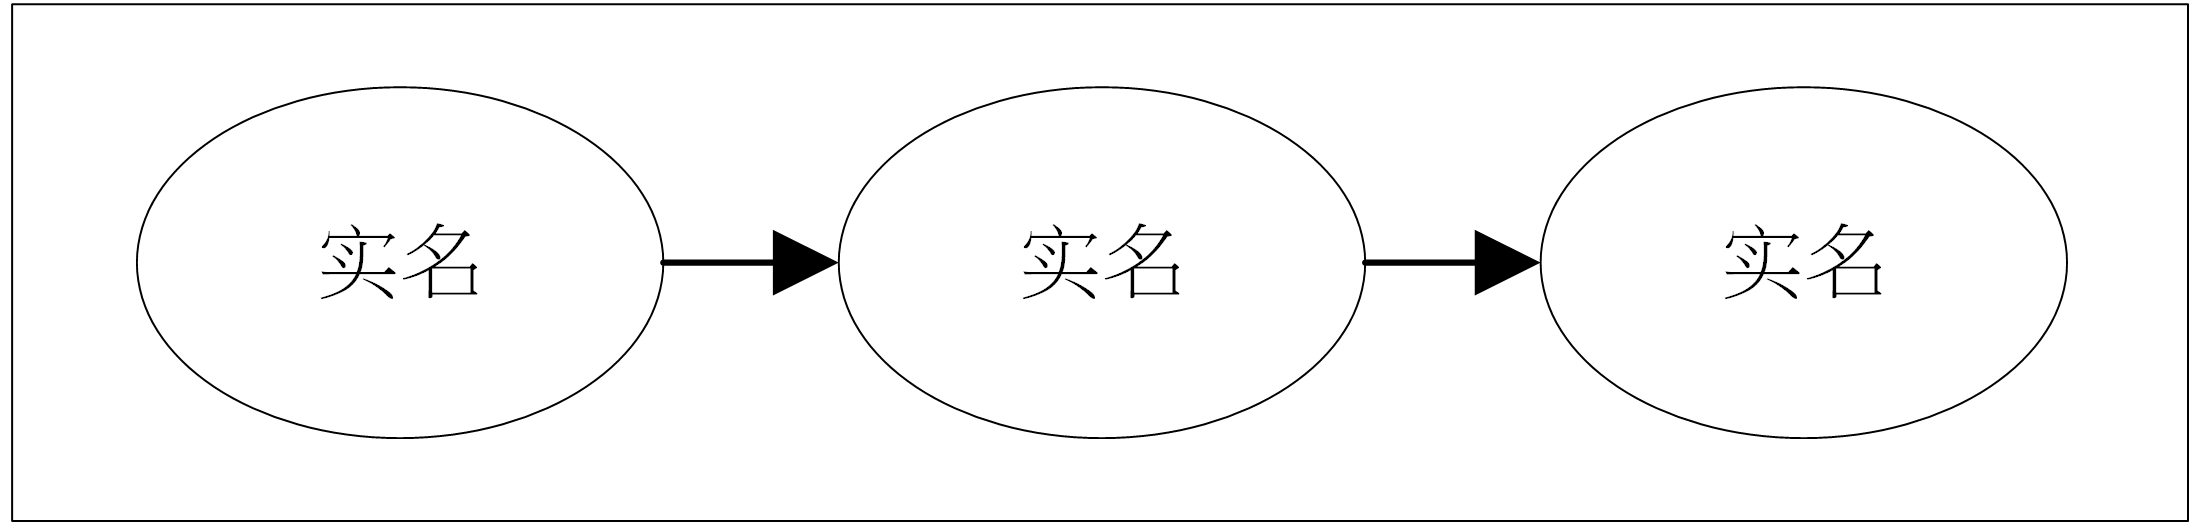
\includegraphics[width = 0.7\textwidth]{modennn.png}
			\caption{實名對實名再對實名交易}\label{modennn}
		\end{figure}

		%%%%%%%fig nnn

		\subsection{實名客戶透過匿名第三方再實名商家}
		為瞭解決在進行交易的過程中使用Visa支付管道會透露太多的消費者個人資訊的問題,PayPal便致力於將消費者的銀行卡相關的個人資訊寄託在PayPal身上,PayPal再以公司的身分,將資金轉移給商家,消費者與店家的交易中間多了一個仲介的角色,也讓這樣的交易模式看似匿名的消費者對上實名的商家。但在這樣的交易過程中,大家的信任需要寄附在PayPal身上,畢竟大部分的銀行卡與個人的資料皆寄託在PayPal公司內,PayPal公司的資訊安全將成為最重要的議題。圖\ref{modenan}為先以實名制的支付管道將資金轉移到代支付的Paypal公司,paypal代為支付的過程中將原資金來源的個人相關資料保護在paypal公司中,以製造出一種匿名支付方法保護消費者的個人資訊的模型。

		\begin{figure}[h]
			\centering
			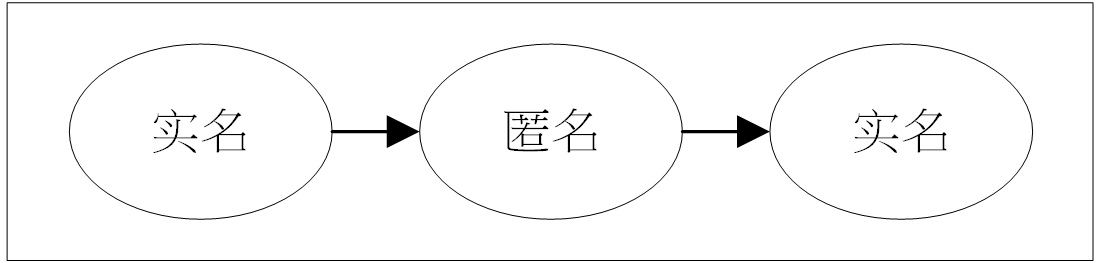
\includegraphics[width = 0.7\textwidth]{modenan.png}
			\caption{實名對匿名再對實名交易}\label{modenan}
		\end{figure}

		%%%%%%%fig ann

%	\section{密碼貨幣交易模型}
%		\subsection{匿名客戶對匿名商家}
%	\section{各種交易模型比較}

% vim:ts=4:sw=4
